\section{113 --- Path Sum II}
Given a binary tree and a sum, find all root-to-leaf paths where each path's sum equals the given sum.

\textbf{Note:} A leaf is a node with no children.

\paragraph{Example:}
 
\begin{flushleft}
\textbf{Input}: Given the below binary tree and \fcj{sum = 22},

\begin{figure}[H]
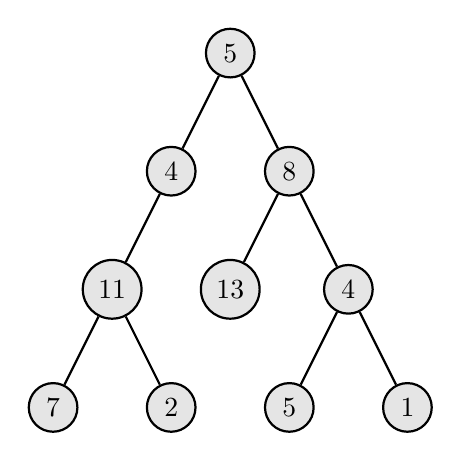
\begin{tikzpicture}
[every node/.style={draw, circle, fill=gray!20!, minimum size=5mm},
%level 1/.style={sibling distance=25mm},
%level 2/.style={sibling distance=15mm},
thick]
\node{5}
child{node{4} child{node{11} child{node{7}} child{node{2}}} child[missing]}
child{node{8} child{node{13}} child{node{4} child{node{5}} child{node{1}} } };
\end{tikzpicture}
\end{figure}
%\begin{figure}[H]
%\begin{tikzpicture}
%[mynode/.style={draw,circle,minimum size=5mm, fill=gray!20!}]
%\node(){};
%\node[mynode](5) {5};
%\node[mynode](4) [below = 8mm of 5, xshift=-15mm] {4};
%\node[mynode](8) [below = 8mm of 5, xshift=15mm] {8};
%\node[mynode](11) [below = 8mm of 4, xshift=-12mm] {11};
%\node[mynode](13) [below = 8mm of 8, xshift=-12mm] {13};
%\node[mynode](41) [below = 8mm of 8, xshift=12mm] {4};
%\node[mynode](7) [below = 8mm of 11, xshift=-8mm] {7};
%\node[mynode](2) [below = 8mm of 11, xshift=8mm] {2};
%\node[mynode](1) [below = 8mm of 41, xshift=8mm] {1};
%\node[mynode](51) [below = 8mm of 41, xshift=-8mm] {5};
%\draw[>=stealth,->] (5) -- (4);
%\draw[>=stealth,->] (5) -- (8);
%\draw[>=stealth,->] (4) -- (11);
%\draw[>=stealth,->] (8) -- (13);
%\draw[>=stealth,->] (8) -- (41);
%\draw[>=stealth,->] (11) -- (7);
%\draw[>=stealth,->] (11) -- (2);
%\draw[>=stealth,->] (41) -- (1);
%\draw[>=stealth,->] (41) -- (51);
%\end{tikzpicture}
%\end{figure}
\textbf{Output}:
\\
$(5,4,11,2)$
\\
$(5,8,4,5)$
\end{flushleft}
\subsection{Recursion}
由于需要保存路径,因此每次进入到递归函数时,将当前node的值插入到当前path的末尾,然后在递归结束时,将末尾的node从path中移除。

\setcounter{lstlisting}{0}
\begin{lstlisting}[style=customc, caption={Backtrace}]
vector<vector<int>> pathSum( TreeNode* root, int sum )
{
    vector<int> path;
    vector<vector<int>> paths;
    dfs( root, sum, path, paths );
    return paths;
}
//helper function for recursive processing
void dfs( TreeNode* node, int sum, vector<int>& path, vector<vector<int>>& paths )
{
    if( !node )
    {
        return;
    }
    if( !node->left && !node->right )
    {
        if( node->val == sum )
        {
            //this is the path
            path.push_back( node->val );
            paths.emplace_back( path.begin(), path.end() );
            //we have to remove for backtrace
            path.pop_back();
        }
        return;
    }
    if( node->left )
    {
        path.push_back( node->val );
        dfs( node->left, sum - node->val, path, paths );
        path.pop_back();
    }
    if( node->right )
    {
        path.push_back( node->val );
        dfs( node->right, sum - node->val, path, paths );
        path.pop_back();
    }
}
\end{lstlisting}